%%%%%
\section{Data Level Methods}
\index{Data Level Methods}

Consider this two-dimensional training dataset, which we will use to illustrate data-level techniques for handling imbalanced datasets.  In real problems, of course, the dataset could have a hundred dimensions and a million samples.  The six blue circles represent samples (elements) of the majority negative class (``no ambulance''), and the three red squares represent the minority positive class (``ambulance'').  


\begin{center}
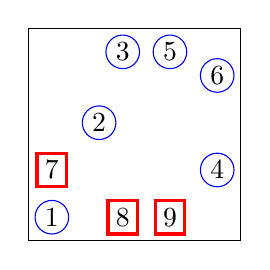
\begin{tikzpicture}[x = 3mm, y=3mm]
	\draw (-1,-1) rectangle (8,8);
	\tikzstyle{Square} = [
		draw = red, 
		very thick,
		rectangle,
		inner sep = 1mm,
		minimum size = 2 mm
	]
	\tikzstyle{SquareFill} = [
		draw = red, 
		fill = red,
		very thick,
		rectangle,
	]
	\tikzstyle{Circle} = [
		draw = blue, 
		circle,		
		inner sep = 0.5mm,
	]
	\tikzstyle{CircleFill} = [
		draw = blue,
		fill = blue, 
		circle,
	]
	\node [Circle] (1) at (0,0) {1};
	\node [Circle] (2) at (2,4) {2};
	\node [Circle] (3) at (3,7) {3};
	\node [Circle] (4) at (7,2) {4};
	\node [Circle] (5) at (5,7) {5};
	\node [Circle] (6) at (7,6) {6};
	\node [Square] (7) at (0,2) {7};
	\node [Square] (8) at (3,0) {8};
	\node [Square] (9) at (5,0) {9};

\end{tikzpicture}
\end{center}

Many algorithms, and variations thereon, have been proposed to balance the two classes before applying a machine learning algorithm to build a model to classify new samples as positive or negative.  WARNING:  Vast oversimplification ahead.  Our goal here is to give the general idea of each method.  


%%%
\subsection{Imbalanced Cleaning:  Tomek and Condensed Nearest Neighbor}
\index{Tomek Links}
\index{Condensed Nearest Neighbor}

Batista
\cite{BATISTA_2004}
uses two imbalanced cleaning method called {\it Tomek links} and {\it Condensed Nearest Neighbor}.  If examples from the majority and minority class are close to each other, it deletes the majority samples.   One could think of it as targeted undersampling of the majority set.  

Imbalanced-Learn, an add-on to Scikit-Learn, has these algorithms read to use.  Tomek and Wilson's papers introducing these algorithms are from the 1970's.  
\index{Imbalanced-Learn}


%%%
\subsection{Tomek's Links}

In 1976, Tomek proposed a method of undersampling that assumes that the majority and minority classes should (at least locally) be clustered. \cite{ivan1976two} If an sample $A$ of the majority class and a sample $B$ of the minority class are each other's nearest neighbors, then one of them is not clustered with its own class.  Since we are trying to undersample the majority class, assume that the element of the majority class is noise (or an error, or just not useful), and delete it.  

In the diagram below, samples \#1 and \#7 are Tomek links, because they are each other's nearest neighbors and of different classes.  Samples \#4 and \#9 are not Tomek links, because while 9 is 4's nearest neighbor, 9's nearest neighbor is 8, not 4.  

In the context of modeling crash severity from police reports, why would sample \#1 not need an ambulance when its characteristics are so close to those of \#7 and not near most of the other crashes without serious injury?  The reason could be errors in the records, or luck/providence/fate.  It could also be that the difference between property damage only and serious injury is influenced by thousands of variables we cannot measure or know, all of the physics of crash forces acting on the bones and structures of the human body.  The best we can say is that the outcome in \#1 cannot be predicted by the information that we have, so that sample will not help in constructing a model based on the available data; therefore, we can reasonably delete it from the training set.  

Tomek's Links can also be run iteratively.  Sample \#7 had \#1 as its nearest neighbor, but once \#1 is deleted, then \#2 and \#7 are each other's nearest neighbors of different classes, thus are Tomek links, and we can delete \#2.  



\begin{center}
\begin{tikzpicture}[x = 3mm, y=3mm]
	\draw (-1,-1) rectangle (8,8);
	\tikzstyle{Square} = [
		draw = red, 
		very thick,
		rectangle,
		inner sep = 1mm,
		minimum size = 3 mm
	]
	\tikzstyle{SquareFill} = [
		draw = red, 
		fill = red,
		very thick,
		rectangle,
	]
	\tikzstyle{Circle} = [
		draw = blue, 
		circle,
		inner sep = 0.5 mm
	]
	\tikzstyle{CircleFill} = [
		draw = blue,
		fill = blue, 
		circle,
	]
	\node [Circle] (1) at (0,0) {1};
	\node [Circle] (2) at (2,4) {2};
	\node [Circle] (3) at (3,7) {3};
	\node [Circle] (4) at (7,2) {4};
	\node [Circle] (5) at (5,7) {5};
	\node [Circle] (6) at (7,6) {6};
	\node [Square] (7) at (0,2) {7};
	\node [Square] (8) at (3,0) {8};
	\node [Square] (9) at (5,0) {9};

	\node [Circle, cross out] (1) at (0,0) {1};
\end{tikzpicture}
\end{center}

%%% Original stuff in Prospectus

This method undersamples the majority-class samples, eliminating ones that are too close to minority-class samples, presuming them to be noise, and helping clarify clusters of minority samples.  

A pair of samples are a {\it Tomek link} if one is majority and one minority, and they are each other's nearest neighbors. To use Tomek's inks as an undersampling strategy for imbalanced data, delete the positive sample in each Tomek's link.  Other cleaning strategies (for balanced sets) would eliminate both the positive and negative.  

It is possible to iterate Tomek's several times.  Here's an example of how it works in one round and in a second round.  The blue samples are from the majority set and the red are from the minority.  Assume that these seven points are a small part of a large dataset, but these are the only points in this region.

\

\noindent\hfil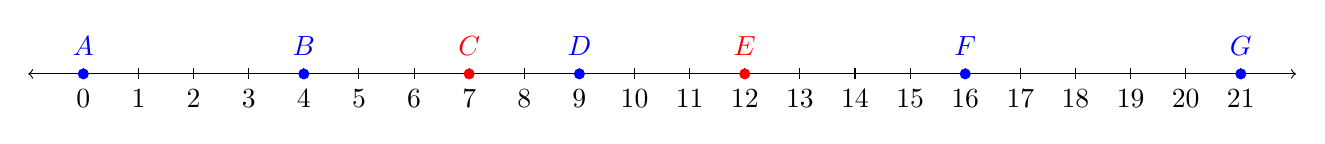
\begin{tikzpicture}[x=7mm, y=7mm]
	\draw [<->] (-1,0) -- (22,0);
	\foreach \x in {0,1,2,...,21}
		\draw (\x, 0.1) -- (\x,-0.1) node [below] {$\x$};
	\fill [blue] (0,0) circle (2pt) node [above=3pt, blue] {$A$};
	\fill [blue] (4,0) circle (2pt) node [above=3pt, blue] {$B$};
	\fill [blue] (9,0) circle (2pt) node [above=3pt, blue] {$D$};
	\fill [blue] (16,0) circle (2pt) node [above=3pt, blue] {$F$};
	\fill [blue] (21,0) circle (2pt) node [above=3pt, blue] {$G$};
	\fill [red] (7,0) circle (2pt) node [above=3pt, red] {$C$};
	\fill [red] (12,0) circle (2pt) node [above=3pt, red] {$E$};
\end{tikzpicture}

In the original dataset, $C$ and $D$ are each other's nearest neighbors, $C$ from minority and $D$ from majority, so they are a Tomek link.   On the other hand, $D$ is the nearest neighbor to $E$, but $E$ is not $D$'s nearest neighbor, so they are not a Tomek link.  

Eliminate sample $D$.  

\

\noindent\hfil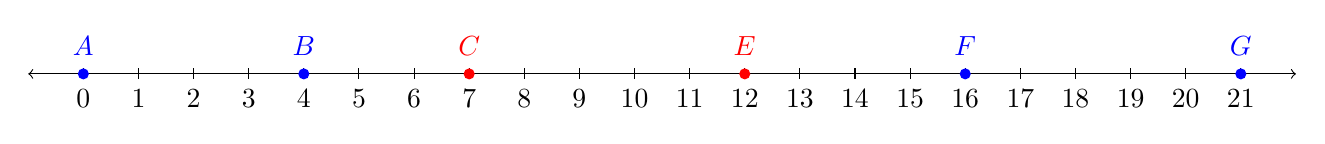
\begin{tikzpicture}[x=7mm, y=7mm]
	\draw [<->] (-1,0) -- (22,0);
	\foreach \x in {0,1,2,...,21}
		\draw (\x, 0.1) -- (\x,-0.1) node [below] {$\x$};
	\fill [blue] (0,0) circle (2pt) node [above=3pt, blue] {$A$};
	\fill [blue] (4,0) circle (2pt) node [above=3pt, blue] {$B$};
%	\fill [blue] (9,0) circle (2pt) node [above=3pt, blue] {$D$};
	\fill [blue] (16,0) circle (2pt) node [above=3pt, blue] {$F$};
	\fill [blue] (21,0) circle (2pt) node [above=3pt, blue] {$G$};
	\fill [red] (7,0) circle (2pt) node [above=3pt, red] {$C$};
	\fill [red] (12,0) circle (2pt) node [above=3pt, red] {$E$};
\end{tikzpicture}

Now the pairs $(B,C)$ and $(E,F)$ are Tomek links, so if we ran Tomek undersampling a second time, we would remove samples $B$ and $F$.  

\

\noindent\hfil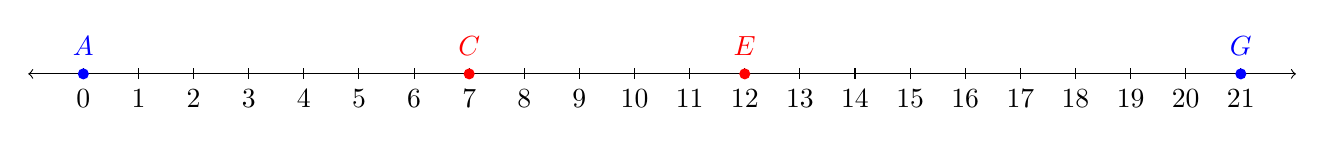
\begin{tikzpicture}[x=7mm, y=7mm]
	\draw [<->] (-1,0) -- (22,0);
	\foreach \x in {0,1,2,...,21}
		\draw (\x, 0.1) -- (\x,-0.1) node [below] {$\x$};
	\fill [blue] (0,0) circle (2pt) node [above=3pt, blue] {$A$};
%	\fill [blue] (4,0) circle (2pt) node [above=3pt, blue] {$B$};
%	\fill [blue] (9,0) circle (2pt) node [above=3pt, blue] {$D$};
%	\fill [blue] (16,0) circle (2pt) node [above=3pt, blue] {$F$};
	\fill [blue] (21,0) circle (2pt) node [above=3pt, blue] {$G$};
	\fill [red] (7,0) circle (2pt) node [above=3pt, red] {$C$};
	\fill [red] (12,0) circle (2pt) node [above=3pt, red] {$E$};
\end{tikzpicture}

Now $C$ and $E$ are each other's nearest neighbors and of the same (minority) class, so this part of the dataset would not change under another run of Tomek.  

The idea of Tomek assumes that the minority samples should cluster, and any majority samples in or near those clusters must be noise, so we can eliminate them.  We now have a clear cluster of two minority samples with no close majority samples.  

I saw multiple runs of Tomek mentioned [somewhere] in my reading, so  I tried it on the crash data, running it up to five times, and saw that it converged, with fewer positive samples eliminated in each round.  I had conjectured that a negative sample in a Tomek link in a later round must have been a negative sample in a Tomek link in an earlier round, digging itself out of a field of positive-class dust, but I suspected that there might be (perhaps unusual) cases where one minority-class sample ($C$ in the example above) created a Tomek link, and eliminating the majority-class sample in that link ($D$ above) allowed a Tomek link for a different minority-class sample ($E$ above).  I then played with it until I found a counterexample to my conjecture, so the conjecture, that a minority-class sample in a Tomek link in a later round of Tomek undersampling must have been in a Tomek link in every previous round of the Tomek undersampling, is false.  

If the conjecture had been true, then we could greatly speed up subsequent rounds of Tomek undersampling by only considering the minority samples in Tomek links in the previous round.  That would not be thorough, but this approach would.  

\subsubsection{Algorithm for Repeated Application of Tomek's Links}

	For the first round of Tomek undersampling, one has to consider each element of the minority class.  In the Tomek's links, call the minority-class elements $\{A_{1}, A_{2}, \dots, A_{n1}\}$, and the majority-class elements $\{B_1, B_2, \dots, B_{n1}\}$.  Tomek undersampling for minority classes eliminates all of $\{B_1, B_2, \dots, B_{n1}\}$.
	
	In the second round of Tomek undersampling, we only need to consider as possible Tomek links the nearest neighbors of $\{A_{1}, A_{2}, \dots, A_{n1}\}$ and any element of the minority class that had one of $\{B_1, B_2, \dots, B_{n1}\}$ as its nearest neighbor.
	
In subsequent rounds, consider the minority-class samples from the Tomek's links from the previous round, and the elements of the minority class that had as their nearest neighbor an element of the majority class in the Tomek's links.  

In theory there could be more Tomek's links in one round than in the previous round, but in practice they go to zero and the set converges to a set with no Tomek's links.  

%%%
\subsection{Cleaning Multiclass Data}
\index{Cleaning Multiclass Data}

Wei (2021) \cite{WEI_2021} uses something similar to Tomek's links for a multi-class problem with a majority class and multiple minority classes.  

\begin{itemize}
	\item Splits an imbalanced multi-class problem with $n+1$ classes ($n$ of them being minority) into $n$ imbalanced binary problems for data cleaning.  
	\item Uses cleaning undersampling (similar to Tomek's Links) to remove noisy spots in the data.
\end{itemize}


%%%
\subsection{Random Oversampling}
\index{Oversampling (Random)}

Random (na\"{i}ve) oversampling creates duplicates of minority class samples until the sets are balanced.  This method has a similar effect to using class weights, introduced below.  

\begin{center}
\begin{tikzpicture}[x = 3mm, y=3mm]
	\draw (-1,-1) rectangle (8,8);
	\tikzstyle{Square} = [
		draw = red, 
		very thick,
		rectangle,
		inner sep = 1mm,
		minimum size = 4 mm
	]
	\tikzstyle{SquareFill} = [
		draw = red, 
		fill = red,`	
		very thick,
		rectangle,
	]
	\tikzstyle{Circle} = [
		draw = blue, 
		circle,
		inner sep = 0.5 mm
	]
	\tikzstyle{CircleFill} = [
		draw = blue,
		fill = blue, 
		circle,
	]
	\node [Circle] (1) at (0,0) {1};
	\node [Circle] (2) at (2,4) {2};
	\node [Circle] (3) at (3,7) {3};
	\node [Circle] (4) at (7,2) {4};
	\node [Circle] (5) at (5,7) {5};
	\node [Circle] (6) at (7,6) {6};
	\node [Square] (7) at (0,2) {7};
	\node [Square] (8) at (3,0) {8};
	\node [Square] (9) at (5,0) {9};

%	\node [Square] (7) at ($(0,2) + (-0.2,-0.2)$) {};
	\node [Square] (8) at ($(3,0) + (-0.2,-0.2)$) {};
%	\node [Square] (9) at ($(5,0) + (-0.2,-0.2)$) {};

%	\node [Square] (7) at ($(0,2) + (0.2,0.2)$) {};
	\node [Square] (8) at ($(3,0) + (0.2,0.2)$) {};
	\node [Square] (9) at ($(5,0) + (0.2,0.2)$) {};


\end{tikzpicture}
\end{center}

Na\"{i}ve oversampling would be to create 99 copies of each of the positive samples, so that the two sets are balanced.  That would have exactly the same effect on the loss function, because there would now be 100 times as many samples with $y_i=1$.  


%%%
\subsection{Undersampling}
\index{Undersampling (Random)}

Random undersampling balances the two classes by randomly deleting elements of the majority class until the two are balanced.  The major drawback of this method is that you throw away information about the majority class.  If the majority class is many more times the size of the minority, you lose almost all of the data.  


\begin{center}
\begin{tikzpicture}[x = 3mm, y=3mm]
	\draw (-1,-1) rectangle (8,8);
	\tikzstyle{Square} = [
		draw = red, 
		very thick,
		rectangle,
		inner sep = 1 mm,
		minimum size = 3 mm
	]
	\tikzstyle{SquareFill} = [
		draw = red, 
		fill = red,
		very thick,
		rectangle,
	]
	\tikzstyle{Circle} = [
		draw = blue, 
		circle,
		inner sep = 0.5 mm
	]
	\tikzstyle{CircleFill} = [
		draw = blue,
		fill = blue, 
		circle,
	]
	\node [Circle] (1) at (0,0) {1};
	\node [Circle] (2) at (2,4) {2};
	\node [Circle] (3) at (3,7) {3};
	\node [Circle] (4) at (7,2) {4};
	\node [Circle] (5) at (5,7) {5};
	\node [Circle] (6) at (7,6) {6};
	\node [Square] (7) at (0,2) {7};
	\node [Square] (8) at (3,0) {8};
	\node [Square] (9) at (5,0) {9};

	\node [Circle, cross out] (1) at (0,0) {1};
	\node [Circle, cross out] (4) at (7,2) {4};
	\node [Circle, cross out] (6) at (7,6) {6};
\end{tikzpicture}
\end{center}


Undersampling would erase 99\% of the negative samples so that the classes would be balanced.  That seems like a bad idea, because you would lose a lot of information about the majority class.  

\subsection{SMOTE:  Synthetic Minority Oversampling TEchnique}
\index{SMOTE}

\acrfull{smote} \cite{00017602530000120020101} is one of the most popular oversampling methods for balancing a dataset with continuous numerical data.  It creates new synthetic minority samples ``between'' original minority samples, not necessarily at the midpoint by choosing a number in $(0,1)$, multiplying the difference (in each dimension) from point $A$ to $B$ by that constant, and adding it to $A$.

In the diagram, the solid red squares represent new synthetic samples between pairs of original minority-class samples.  SMOTE does not consider the positions of the majority-class samples, only considering the difference in number of nodes to bring the two classes closer to parity.  

\begin{center}
\begin{tikzpicture}[x = 7mm, y=7mm]
%	\draw (-1,-1) rectangle (8,8);
	\tikzstyle{Square} = [
		draw = red, 
		very thick,
		rectangle,
		minimum size = 5 mm
	]
	\tikzstyle{Synth} = [
		draw = red, 
		fill = red,
		very thick,
		rectangle,
		minimum size = 3mm
	]
	\tikzstyle{Circle} = [
		draw = blue, 
		circle,
	]
	\tikzstyle{CircleFill} = [
		draw = blue,
		fill = blue, 
		circle,
	]
	\node [Square] (7) at (0,2) {7};
	\node [Square] (8) at (3,0) {8};
	\node [Square] (9) at (5,0) {9};

	\draw (7) -- (8);
	\draw (7) -- (9);
	\draw (8) -- (9);
	
	\node [Synth] () at ($0.3*(7) + 0.7*(8)$) {};
	\node [Synth] () at ($0.7*(7) + 0.3*(9)$) {};
	\node [Synth] () at ($0.5*(8) + 0.5*(9)$) {};


\end{tikzpicture}
\end{center}

One challenge with SMOTE is that it is only useful for datasets with continuous numerical data, and our data is almost all categorical.  What is between ``car'' and ``school bus,'' or between ``parking lot'' and ``highway''?  SMOTE has a variant, SMOTE-NC (Nominal and Continuous) that can handle datasets with some nominal (categorical) features, but most of the features need to be continuous; thus, we will not be able to use SMOTE or similar techniques for our work.  

%%% Original stuff in Prospectus

Especially if we're doing fatalities, we have a terribly imbalanced data set.  Ideally we'd like to have an equal number of fatal and nonfatal crashes to plug into our ML algorithm, but we have about 0.47\% fatal and 99.53\% nonfatal.  

One solution is to randomly choose 681 nonfatal crashes to compare with our 681 fatal crashes, but that leaves behind a LOT of information.  

Many of the papers I've read use SMOTE, which balances the data set by creating synthetic elements for the minority set (fatal crashes).  It picks an element of the minority set, $a$, and picks one of its nearest neighbors, $b$, and creates a new synthetic element $c$.  For each data category, $D_i$, in which they differ, SMOTE chooses $D_i(c)$ to be between $D_i(a)$ and $D_i(b)$.  It randomly chooses a random number $r \in [0,1]$, and makes $D_i(c) = D_i(a) + r(D_i(a) - D_i(b))$.  

I get how that works for continuous variables.  I get that it would work if $D_i(a)$ and $D_i(b)$ weren't very different.  

How would that work for boolean variables?  SMOTE would choose nearest neighbors $a$ and $b$ that agree on most variables, but for values of $i$ where $D_i(a)=0$ and $D_i(b)=1$, it would randomly choose $D_i(c) \in \{0,1\}$.  There is no {\it between} for boolean variables.  It doesn't seem to me that it would work as well.  

Original SMOTE only works with continuous variables.  There is something called SMOTE-NC that handles continuous and categorical, but it has to have some continuous variables to work on.  

\begin{quote}
Unlike SMOTE, SMOTE-NC for dataset containing numerical and categorical features. However, it is not designed to work with only categorical features.
\end{quote}

\url{https://imbalanced-learn.org/dev/references/generated/imblearn.over_sampling.SMOTENC.html}

Since we have $\approx 200$ times as many nonfatal crashes as fatal crashes, to balance the data set with SMOTE, we would have to make two hundred synthetic elements for each fatal crash.  It seems to me that we would be making a mess of our data set.  
		


%%%
\subsection{Flavors of SMOTE}
\index{SMOTE Flavors}

SMOTE, or Synthetic Minority Oversampling TEchnique, 			\cite{CHAWLA_2002}
 creates extra samples of the minority class, but rather than making exact copies, it finds two similar samples and creates more samples ``between'' them, with feature values between the values of the two samples.  SMOTE only works for continuous features, not for categorical features.  Almost all of my features are categorical.  
 
 I got this list of flavors of SMOTE from a 2021 review by Mahmudah.
			\cite{MAHMUDAH_2021}  I've investigated some of them and given some flesh to some parts of this skeleton.
 
 		\begin{itemize}
			\item SMOTE:  Synthetic Minority Oversampling TEchnique 
			\cite{CHAWLA_2002}
			
			Uses $k$-nearest neighbors to find two close positive (minority) samples, and creates a synthetic sample between them.  Works on continuous data, not on categorical or binary data.  
			
			\item ADASYN:  ADAptive SYNthetic sampling approach for imbalanced learning.  
			\cite{MAHMUDAH_2021}
			
			Creates synthetic samples based on the level of difficulty in learning the samples of the minority class.  A positive samples is ``difficult'' if it has more negative samples as its nearest neighbors.  The more difficult a sample is, the more synthetic copies of that sample ADASYN creates.  
			
			\item Borderline SMOTE
			\cite{MAHMUDAH_2021}
			
			Generates synthetic positive samples along the border between the positive and negative classes.  Brad's Question:  This assumes you know where the border is.  I suppose you could do it iteratively.  
			
			\item Safe-level SMOTE
			\cite{MAHMUDAH_2021}

			When SMOTE finds the nearest positive-class neighbors of a positive sample, it ignores the negative (majority-class) neighbors.  [I think this is what it means:]  Creating synthetic positive-class samples in a neighborhood with lots of negative samples just makes more of a mess, so this is not considered a ``safe'' place to make synthetic samples.  Safe-level SMOTE creates synthetic positive samples only in majority-positive neighborhoods.  
			
			\item Relocating-safe-level SMOTE (RSLS)
			\cite{MAHMUDAH_2021}
			
			Avoids creating synthetic positive samples near negative samples.  
			
			\item Density-based SMOTE (DBSMOTE)
			\cite{MAHMUDAH_2021}

			Integration of DBSCAN and SMOTE.   DBSCAN, Density-Based Spatial Clustering of Application with Noise, discovers clusters with an arbitrary shape (?)  DGSMOTE creates synthetic samples at the pseudo-centroids of the clusters of positive samples.  
			
			\item Adaptive Neighbor SMOTE (ANS)
			\cite{MAHMUDAH_2021}

			Focuses not on -where- to generate synthetic samples, but on -how many- samples to generate in a particular neighborhood. 

			\item D2GAN 

This 2020 article by Zhai \cite{ZHAI_2020_D2GAN} builds on the Dual Discriminator Generative Adversarial Nets (D2GAN) paper from 2017 by Nguyen \cite{NGUYEN_2017}.  They want to do better oversampling, comparing D2GAN with SMOTE.  I don't understand what this is, but they say SMOTE has three drawbacks:

\begin{enumerate}
	\item Ignores the probability distribution of minority class samples.
	\item Synthetic examples lack diversity.
	\item Interating SMOTE many times will give synthetic samples with significant overlap.
\end{enumerate}

This 2022 article by Zhai \cite{ZHAI_2022} slightly modifies Zhai's claims against SMOTE.

\begin{enumerate}
	\item Does not extend the training field of positive samples.
	\item Synthetic examples lack diversity.
	\item Does not accurately approximate the probability distribution of minority class samples.
\end{enumerate}

The authors propose two new methods of diversity oversampling by generative models, one based on ``extreme machine learning autoencoder,'' and the other based on generative adversarial networks (GAN).  

			
		\end{itemize}
		
%%%
\subsection{Oversampling Image Data}
\index{Oversampling Image Data}

Extracting knowledge from a database of tabular numerical or categorical data is difficult, but a database of images is a challenge of a different magnitude.  An imbalanced labeled image dataset for crash prediction modeling might be a thousand images taken ten seconds before a crash and a million images taken ten seconds before ... nothing happened.  Deep neural networks (DNN) and (deep) convolutional neural networks (DCNN and CNN) are common methods for image data.  \cite{NIPS2014_5ca3e9b1} introduced Generative Adversarial Networks, which can be used to generate synthetic samples to balance the dataset.  Given the power of the tools for image recognition, many researchers make non-image data look (to the computer) like images to take advantage of the tools.  



%%%
\subsection{Train/Test Split}
\index{Train/Test Split}

The application in Sharififar's 2019 article \cite{SHARIFIFAR_2019}  is digital mapping of farmland, categorizing areas by soil type.  Some soil types are rare but significant.  This is the first article I've seen that, at the beginning, says that making sure each minority class appears in appropriate distribution in the validation and test sets is an important challenge.  They explicitly say that they split 30\% for the validation set by taking 30\% of each class.

%%%
\subsection{Feature Selection}
\index{Feature Selection}

This 2012 article by Tan \cite{TAN_2012} introduces a feature selection model specifically for imbalanced data sets.  I haven't dug in yet.  


